%======================================================================
\section{Dónde puede actuar una capa de riesgo}\label{sec:riesgo-donde}
%======================================================================
\paragraph{Qué se busca.} Los escenarios extremos (sección~\ref{sec:extremos}) dejaron una
pregunta abierta. Con la caja archivada el MPC siempre satura, y con el actuador físico el
límite de 1220~K queda lejos. En ninguno de los dos casos una capa de riesgo puede cambiar una
decisión. Antes de diseñarla hay que ubicar el régimen en que el MPC tiene decisiones libres
\emph{y} la seguridad está en juego, y corregir lo que el gemelo no sabe.

\paragraph{Un cambio en la planta.} La capacidad del ACS (\code{acs\_max}), su rampa
(\code{acs\_ramp}) y su eficiencia $\eta$ (\code{acs\_eta}) pasan a ser parámetros de la réplica
del HRM, y limitan por igual a quien mueva la bomba: el MPC, el PI del DET o el PID de la tesis.

%----------------------------------------------------------------------
\subsection{El mapa de capacidad}
%----------------------------------------------------------------------
Familia extrema (14 realizaciones), $\dot m_{\max}\in\{15,\dots,70\}$~kg/s y rampas de
2.5--10~kg/s por paso; N2+sesgo frente al PI del DET con la misma capacidad y la misma $\eta$
(\code{julia/f5b1a\_capacity\_sweep.jl}).

\begin{figure}[H]\centering
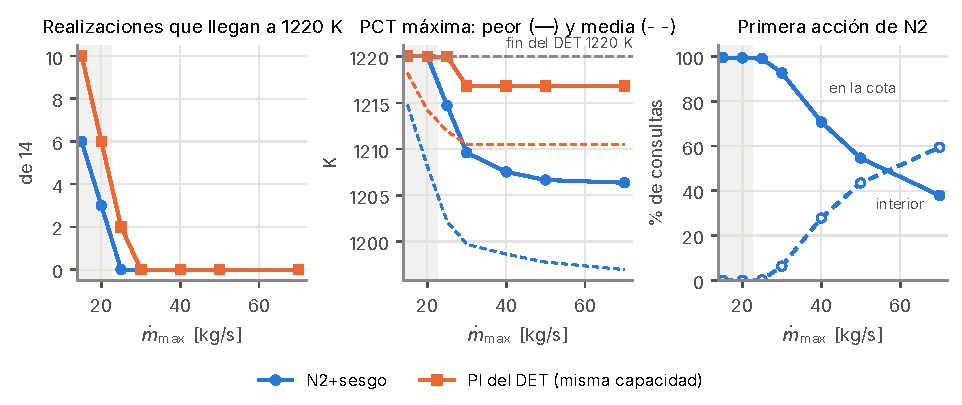
\includegraphics[width=\linewidth]{figures/fig_f5b_capacity_map.pdf}
\caption{Mapa de capacidad (rampa 5~kg/s por paso). Con $\le20$~kg/s, N2 está siempre en la
cota y llega a 1220~K en 3--6 de 14 realizaciones; el PI, en 6--10. Con $\ge40$~kg/s, N2
decide en el interior el 28--60\,\% de las veces y no hay riesgo.}
\end{figure}

\begin{figure}[H]\centering
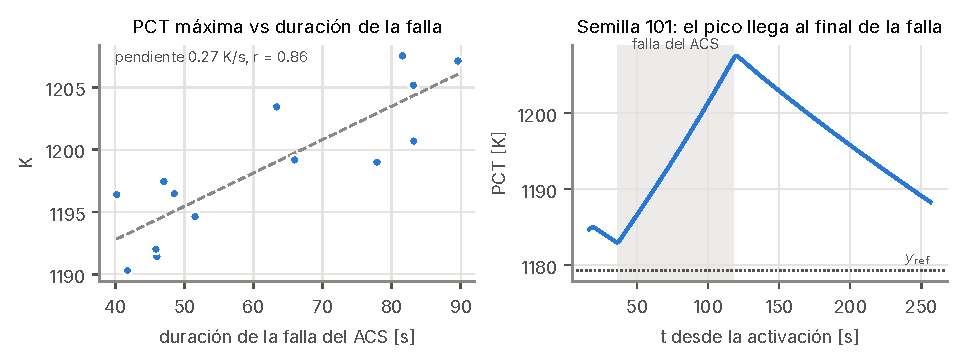
\includegraphics[width=\linewidth]{figures/fig_f5b_peak_at_failure.pdf}
\caption{De dónde sale el pico: la PCT máxima llega siempre al final de la falla del ACS, y
crece con su duración ($\approx0.3$~K/s, $r=0.86$).}
\end{figure}

\noindent La segunda figura es la observación clave de toda esta parte. Durante una falla el
caudal es cero, decida lo que decida el MPC: la PCT sube a $\approx0.3$~K/s hasta que el ACS
vuelve. El pico es entonces la PCT al empezar la falla \emph{más} un calentamiento que sólo
depende de cuánto dura la falla. Esa estructura aditiva se formaliza en la
sección~\ref{sec:prop-aditiva}.

%----------------------------------------------------------------------
\subsection{Lo que el gemelo no sabe}
%----------------------------------------------------------------------
\begin{itemize}
  \item \textbf{Pronóstico de fuga sin la ley de Park.} Un filtro de Kalman de tendencia
        lineal local (nivel y pendiente), con intervención ante saltos de la rotura, es 5--10
        veces más preciso que la persistencia con ruido de medición y tiene la cobertura
        calibrada (\code{python/f5b0\_leak\_forecast.py}). Sin la intervención, no se
        recupera de un salto.
  \item \textbf{Caudal medido del ACS.} El gemelo puede usar el caudal que la planta recibió de
        verdad en lugar del pedido, de modo que sabe cuándo el ACS falló.
  \item \textbf{En lazo cerrado ninguna de las dos cosas importa.} El pronosticador y el caudal
        medido cambian las decisiones (hasta 4~kg/s), pero no la PCT: las diferencias pareadas
        son $0.00\pm0.00$~K en 14 realizaciones, con y sin saltos. La inercia térmica filtra las
        diferencias de caudal, y la corrección de sesgo absorbe el resto.
\end{itemize}
Los márgenes deterministas (DSM) tampoco cambian la PCT máxima, ni en la familia extrema ni en
los escenarios de la tesis (sección~\ref{sec:dsm-lambda}).

\takeaway{El régimen «decisión libre y con riesgo» está vacío en la familia extrema. Donde
hay riesgo, el actuador ya está saturado; donde hay capacidad libre, las fallas de 30--90~s no
alcanzan a llevar la PCT a 1220~K. El pico lo fija la duración de la falla, así que la única
palanca de una capa de riesgo es \emph{pre-enfriar} antes de una falla posible. Para que esa
palanca importe hace falta un modelo de fallas con cola: fallas lo bastante largas, con una
probabilidad conocida.}

%======================================================================
\section{Fallas como en el árbol de eventos y una cota de riesgo}\label{sec:riesgo-cota}
%======================================================================
\paragraph{El modelo de fallas del DET.} El ACS tiene 5 componentes en serie, y cada uno es
una cadena de Markov operativo $\leftrightarrow$ fallado, con tasa de falla $\lambda_i$ y de
reparación $\mu_i$ (\code{msfcn\_indirectps\_hrm\_c.c},
\code{MCDET\_conferencepaper\_database.mat}). El sistema falla si falla cualquier componente.
Por eso las fallas del sistema llegan como un proceso de Poisson de tasa
$\lambda=\sum_i\lambda_i$, y la duración $D$ de una falla es una mezcla de exponenciales:
\[
S(t)=P(D>t)=\sum_i w_i\,e^{-\mu_i t},\qquad w_i=\lambda_i/\textstyle\sum_j\lambda_j .
\]
La exponencial no tiene memoria: una falla que ya lleva 60~s tiene la misma distribución de lo
que le falta que una recién empezada (dentro de cada componente). Con las tasas reales, una
falla en 240~s tiene probabilidad $\approx4\cdot10^{-6}$ y dura días, y ningún controlador puede
evitar los 1220~K. Por eso se usa la opción acelerada que el propio modelo trae comentada
($\lambda\times10^5$, $\mu\times10^4$): las fallas llegan a razón de $1.6\cdot10^{-3}$~s$^{-1}$ y
duran según una mezcla con medias de 46, 46, 25 y 6.5~s y una componente de 2.9~h con peso
0.002 (mediana 29~s; 5.7\,\% dura más de 130~s). Las realizaciones se condicionan a que haya al
menos una falla en la ventana del MPC, igual que el DET ramifica en el evento de falla. La
sección~\ref{sec:riesgo-aplicabilidad} discute qué significa físicamente esta aceleración.

\begin{figure}[H]\centering
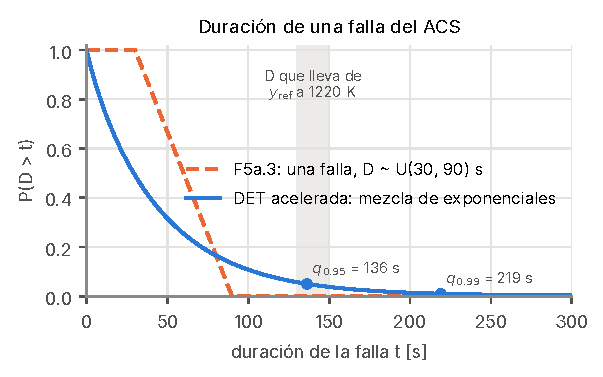
\includegraphics[width=0.62\linewidth]{figures/fig_f5b_failure_duration.pdf}
\caption{Duración de una falla. La familia extrema de F5a.3 nunca pasaba de 90~s; la del DET
tiene cola, y en esa cola está el riesgo de llegar a 1220~K.}
\end{figure}

\paragraph{La cota de riesgo.} Se quiere que una falla que empieza ahora no lleve la PCT sobre
1220~K, salvo con probabilidad $\alpha$. En cada consulta, el ROM simula «el ACS falla ahora y
la fuga sigue» durante $q_{1-\alpha}(D)$ segundos, el cuantil de la duración, y obtiene el
calentamiento $\Delta T(q_{1-\alpha})$ (\code{heatup\_curve}, incluido el salto de $p_4$ al
cortarse el caudal). N2 mantiene entonces
\[
\hat y_k+d\le U_\alpha:=1220-\Delta T\big(q_{1-\alpha}(D)\big),
\]
con una holgura penalizada en norma $\ell_1$ exacta, de modo que sigue siendo un QP. Valores
típicos: $U_\alpha\approx1191$, 1181, 1169 y 1159~K para $\alpha=0.10$, 0.05, 0.02 y 0.01. Es un
\emph{back-off} derivado del proceso de fallas, no del error de pronóstico. La
sección~\ref{sec:prop-aditiva} demuestra que esta cota equivale exactamente a la restricción
$P(\text{cruce}\mid\text{falla ahora})\le\alpha$.

\paragraph{Una corrección en el camino.} En una primera versión, la holgura era cuadrática.
Con cotas inalcanzables ($\alpha=0.01$ y fugas de 25~kg/s, $U_\alpha\approx1090$~K) el QP quedaba
mal escalado: Clarabel falló en 11 corridas y una llegó a 1220~K por aplicar un plan inválido.
Con la penalización $\ell_1$ ($\lambda_r=10^3$~K$^{-1}$) y, si el QP no termina en un óptimo, el
plan anterior desplazado, hubo 0 fallas del solver.

\begin{table}[H]\centering\footnotesize\setlength{\tabcolsep}{4pt}
\begin{tabularx}{\linewidth}{@{}Y r r r r r@{}}\toprule
Caso (60 realizaciones) & Llegan a 1220~K & Peor PCT & $\Delta$ PCT máx.\ vs N2 & ISE / ISE(N2) & Masa extra\\\midrule
N2+sesgo & 0 & 1218.5~K & --- & 1.00 & ---\\
N2+cota, $\alpha=0.05$ & 0 & 1212.0~K & $-1.1\pm0.6$~K & 0.81 & +2\,\%\\
N2+cota, $\alpha=0.02$ & 0 & 1212.0~K & $-4.0\pm1.3$~K & 2.58 & +17\,\%\\
N2+cota, $\alpha=0.01$ & 0 & 1212.0~K & $-5.0\pm1.6$~K & 6.45 & +33\,\%\\
PI del DET & 7 & 1220.1~K & $+20.1\pm1.4$~K & 8.8 & +19\,\%\\\bottomrule
\end{tabularx}
\caption{Cota de riesgo con fallas como en el DET (40~kg/s, rampa 5; \code{julia/f5b1c\_risk.jl}).
Cada realización tiene al menos una falla.}
\end{table}

\begin{figure}[H]\centering
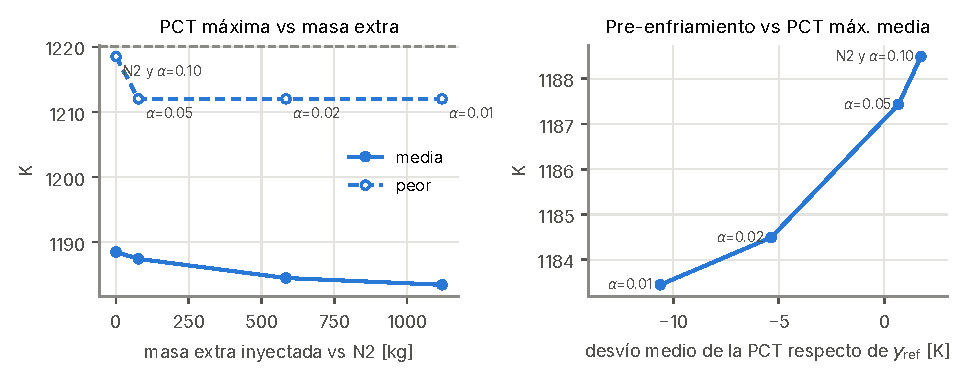
\includegraphics[width=\linewidth]{figures/fig_f5b_risk_frontier.pdf}
\caption{Frontera costo--riesgo de la cota. $\alpha=0.05$ baja la peor PCT 6.5~K y reduce el
ISE; con $\alpha\le0.02$ se paga con pre-enfriamiento.}
\end{figure}

\paragraph{Cómo leer la tabla.}
\begin{enumerate}
  \item \textbf{Ninguna versión de N2 llega a 1220~K}; el PI del DET llega en 7 de 60.
  \item \textbf{Lo que la cota sí cambia es el margen.} Con $\alpha\le0.05$, la peor PCT baja de
        1218.5 a 1212.0~K: en la realización 208 (fuga de 24.7~kg/s y una falla de 118~s), la
        cota mantiene la PCT bajo $U_\alpha$ antes de la falla y eso compra 6.5~K.
  \item \textbf{$\alpha=0.05$ sale casi gratis.} $U_\alpha\approx1181$~K está casi en la
        consigna: el pre-enfriamiento es mínimo y acorta el sobrepaso después de las fallas,
        que es lo que domina el ISE (que baja un 19\,\%).
  \item \textbf{Con $\alpha\le0.02$ se paga}: el MPC trabaja 5--11~K bajo la consigna, y el ISE
        sube de 2.6 a 6.5 veces.
  \item \textbf{Contar cruces no alcanza.} Con 0 cruces en 60 realizaciones, la probabilidad de
        N2 sólo queda acotada bajo el 6\,\%, y las variantes no se pueden comparar. Hace falta
        un estimador de menor varianza (sección~\ref{sec:riesgo-rb}).
\end{enumerate}

\takeaway{\textbf{Respuesta a Q9.} El riesgo de llegar a 1220~K está en las fallas largas del
ACS: el pico llega al final de la falla y crece con su duración. Con fallas como en el DET, una
cota sobre la PCT, derivada del cuantil de la duración, mantiene un margen calibrado y sigue
siendo un QP.}
